\documentclass[11pt]{article}
\usepackage[scaled=0.92]{helvet}
\usepackage{geometry}
\geometry{letterpaper,tmargin=1in,bmargin=1in,lmargin=1in,rmargin=1in}
\usepackage[parfill]{parskip} % Activate to begin paragraphs with an empty line rather than an indent %\usepackage{graphicx}
\usepackage{amsmath,amssymb, mathrsfs, dsfont}
\usepackage{mathtools}

\usepackage{tabularx}
\usepackage[font=footnotesize,labelfont=bf]{caption}
\usepackage{graphicx}
\usepackage{xcolor}
%\usepackage[linkbordercolor ={1 1 1} ]{hyperref}
%\usepackage[sf]{titlesec}
\usepackage{natbib}
\usepackage{../../Tianpei_Report}

%\usepackage{appendix}
%\usepackage{algorithm}
%\usepackage{algorithmic}

%\renewcommand{\algorithmicrequire}{\textbf{Input:}}
%\renewcommand{\algorithmicensure}{\textbf{Output:}}



\begin{document}
\title{Lecture 8: On-policy Prediction with Function Approximation}
\author{Tianpei Xie}
\date{ Aug 10th., 2022 }
\maketitle
\tableofcontents
\newpage
\section{Introduction}
In this chapter, we begin our study of function approximation in reinforcement learning by considering its use in estimating the state-value function from on-policy data, that is,
in approximating $v_{\pi}$ from experience generated using a known policy $\pi$. 

There are two groups of RL methods based on how the value function are represented and stored
\begin{itemize}
\item \emph{\textbf{Tabular} methods}: The value function is stored as a table, i.e. for each $s$, there is a value $v(s)$ (or $q(s,a)$ for each pair $(s,a)$ ) in the table. The tabular representation has good \textbf{discriminization} but no \textbf{generalization}. In other words, value for each state is stored and updated \textbf{independently}, so the dimension of the representation for the tabular value function is $|\cS|$ for $v$ and $|\cS| \times |\cA|$ for $q$. Also it cannot be applied to applications where the total set of states $|\cS|$ is large. 

\item \emph{\textbf{Function approximation} methods}: The value function is \emph{\textbf{parameterized}}. The function approximation allows us to represent the value function via its low dimensional paramater $d \ll |\cS| $, which is more \emph{efficient} in representation and storage, esp. when state-space $\cS$ is very large. On the other hand, the value for \emph{all} states are affected by the change of parameter. It will reduce the  \textbf{discriminization} in order to gain \textbf{generalization}. As its name suggests, the value function estimated via function approximation is not exact but approximation.
\end{itemize}

\begin{figure}
\begin{minipage}[t]{1\linewidth}
  \centering
  \centerline{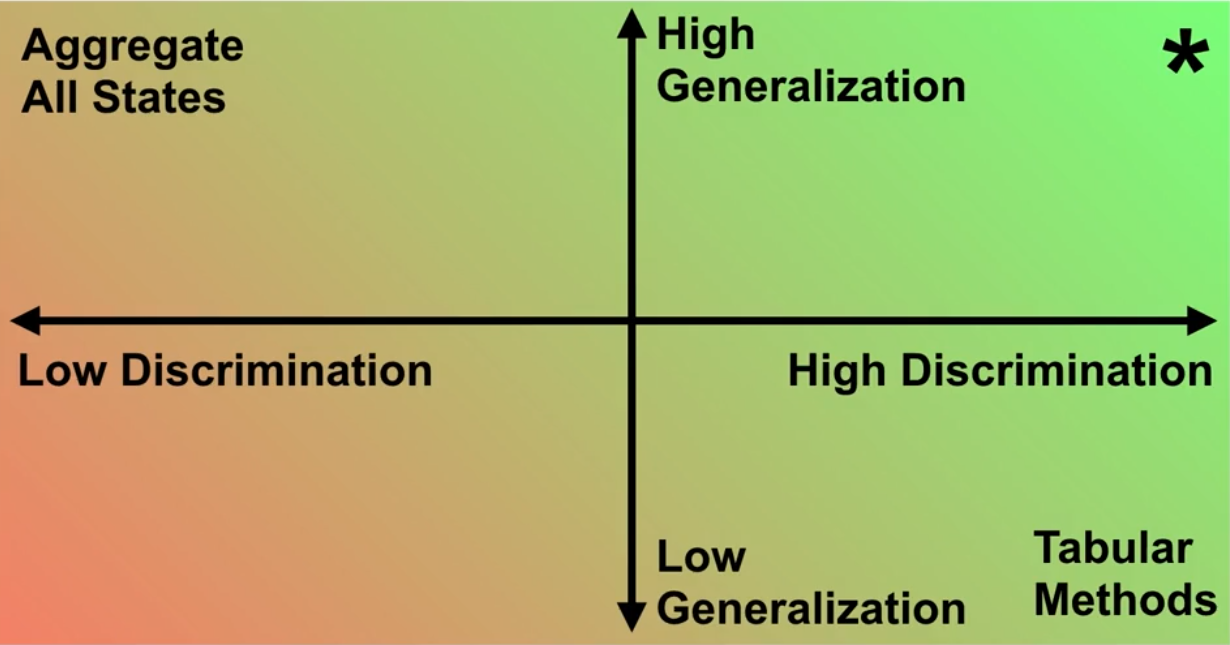
\includegraphics[scale = 0.2]{generalization_discrimination.png}}
\end{minipage}
\caption{\footnotesize{\textbf{Generalization and discrimination are two independent dimensions to evaluate a value estimation strategy.}}}
\label{fig: generalization_discrimination}
\end{figure}

In discussion above, we listed out two important concepts for value estimation:
\begin{itemize}
\item  \textbf{\emph{Generalization}}, which means updating value of one state would affect the value of other states. That is, the change \emph{\underline{generalizes}} from that state to affect the values of many other states. Aggregate all states would easily achieve high generalization but with no discrimination. 

\item \textbf{\emph{Discriminization}}, which means the ability to make the value of two states different. If value of each states are represented independently, such as tabular methods, the discrimination is maximized but there is no generalization. 
\end{itemize} A good value estimation method need to have good generalization and good discrimination. 

\section{Value-function approximation as supervised learning}
\emph{\textbf{Value-function approximation}} problem can be treated as a \textbf{supervised learning problem}. Note that in supervised learning, we are given a set of covariates-target pairs $\set{(s_{t}, G_{t})}_{t=1, \ldots, T}$, the problem is to estimate the function $v: \cS \rightarrow \bR$ so that $\| G_{t} - v(s_{t})\|_{2}^{2}$ is small in expectation. 

In RL, the \emph{\textbf{target}} is defined as the \emph{\underline{expected returns}} or its \textbf{approximation}. The \textbf{covariates} are states or state-action pairs. Given the functional form of value function $v(s, \mb{w})$, we listed out the target definition of several important algorithms 
\begin{itemize}
\item \textbf{Expected returns (Ground Truth)}: $$v_{\pi}(s_{t}):= \E{\pi}{G_{t} | S_{t} = s_{t}}.$$ The ground truth target is the expected returns given state $s_{t}$ and policy $\pi$ and dynamic $p(s', r| s, a)$.  

\item \textbf{Boostrapped expected returns (Dynamic Programming)}: $$v_{\pi}(s, \mb{w}_{t}) :=  \E{\pi}{R_{t+1}  + \gamma\,v_{\pi}(S_{t+1}, \mb{w}_{t}) | S_{t} = s}.$$ The target depends on expected estimate of next rewards, the expected estimate of value for all next states. 


\item \textbf{Sample returns (Monte Carlo methods)}: $G_{t}$, obtained by sampling the entire episode starting at $S_{t}$ and averaging all rewards in the process.

\item \textbf{Boostrapped sample returns (Temporal difference methods)}: $$\hat{G}_{t} := R_{t+1} + \gamma v_{\pi}(S_{t+1}, \mb{w}_{t}),$$ i.e. the target depends on both the next rewards and the value estimate of next state.
\end{itemize}

Using supervised learning for prediction/policy evaluation task has several challenges:
\begin{itemize}
\item Conventional supervised learning assumes the samples follow some \textbf{static distribution} and are \textbf{independent} identically distributed (i.i.d.). In general, this is not satisified in RL setting. Note that all sample pair $(S_{t}, G_{t})$ are generated by some Markove Decision Process, which are natrually \textbf{correlated}. 

\item The underlying \textbf{distribution of sample} in conventional supervised learning is fixed, \textbf{stationary}, unknown. But in RL, there is no assumption on the distribution for each state-action pair within the MDP. In fact, in typical use case of RL, the environment is \textbf{dynamic}, thus the underlying distribution of states is changing.

\item The \textbf{target function} of conventional supervised learning is  fixed. In RL such as TD methods or DP methods, the target function is determined by the value estimation of successor states, which is \textbf{non-stationary} and changing according to the change of value estimation.

\item RL methods need to do \textbf{online learning}.  In reinforcement learning, it is important that learning be able to occur online, while the agent
interacts with its environment or with a model of its environment. To do this requires methods that are able to learn efficiently from \emph{incrementally acquired} data.
\end{itemize}

\subsection{The objective of prediction}
The objective function for value approximation uses the \textbf{Mean Squared Value Error}, denoted $\overline{VE}$:
\begin{align*}
\overline{VE}(\mb{w}) &= \sum_{s \in \cS}\mu(s)\norm{v_{\pi}(s) - \hat{v}(s, \mb{w})}{2}^{2}
\end{align*} where $v_{\pi}(s)$ is the target value function, and $\hat{v}(s, \mb{w})$ is the learned approximated value function. The \textbf{\emph{state distribution}} $\{\mu(s)\} \subset \Delta$ helps to balance the generalization and discrimination. By assumption we have far more states than weights, so making one state’s estimate more accurate invariably means making others’ less accurate. We are obligated then to say which states we \textbf{care most} about. Often $\mu(s)$ is chosen to be the \textbf{fraction of time} spent in $s$. Under on-policy training this is called the \textbf{on-policy distribution}; we focus entirely on this case in this chapter. In continuing tasks,
the on-policy distribution is the \textbf{\emph{stationary distribution}} under $\pi$. In Markov chain theory, $\mu(s)$ is the \textbf{stationary distribution} of Markov Chain, or we called it \textbf{steady-state distribution}.

Note that in episodic task, the on-policy distribution $\mb{\mu}$ can be selected by equations:
\begin{align*}
\eta(s') &= h(s') + \sum_{s}\eta(s) \sum_{a}\pi(a|s)p(s'|s, a), \quad \text{for all } s'\in \cS \\
\mu(s') &= \frac{\eta(s')}{\sum_{s}\eta(s)}
\end{align*} where $h(s)$ denote the probability that an episode \textbf{begins in each state} $s$, and $\eta(s)$ denote the number of time steps spent, on average, in state $s$ in a single episode. This formular indicates that the on-policy distribution $\mb{\mu}$ is a function of policy $\pi(a|s)$. In this chapter, the policy $\pi$ is fixed, therefore $\mb{\mu}$ is constant state weight. In future chapters for policy gradient, when the policy  $\pi(a|s)$ is changing, this distribution will also change. 

Unlike supervised learning, the \textbf{goal} of RL is to learn the \textbf{optimal policy} instead of optimal value function. For many nonlinear functions, finding the ideal \textbf{global optimal} $\mb{w}_*$ so that $\overline{VE}(\mb{w}_*) \le \overline{VE}(\mb{w})$ for all $\mb{w}$ is not easy. Instead, the function approximation algorithm would converge to some \textbf{local minimal}.

\section{Stochastic gradient and semi-gradient methods}
To solve the minimization problem on $\overline{VE}(\mb{w})$, we simply apply the \textbf{stochastic gradient descent (SGD)} algorithm:
\begin{align*}
\mb{w}_{t+1} &\leftarrow \mb{w}_{t} - \frac{1}{2}\alpha \grad{\mb{w}}{\overline{VE}( \mb{w}_{t})} \\
&=  \mb{w}_{t} + \alpha (v_{\pi}(S_{t}) - \hat{v}(S_{t}, \mb{w}_{t})) \grad{\mb{w}}{\hat{v}(S_{t}, \mb{w}_{t})} \\
&= \mb{w}_{t} + \alpha\delta_{t} \grad{\mb{w}}{\hat{v}(S_{t}, \mb{w}_{t})} 
\end{align*} The term $\delta_{t}:= (v_{\pi}(s) - \hat{v}(s, \mb{w}_{t})) $ defines the \textbf{error} i.e. the difference between target value and the approximation function and the second term $\grad{\mb{w}}{v(s, \mb{w}_{t})}$ finds the gradient of the value function. The SGD algorithm is preferred since in many cases, we do not seek or expect to find a value function that has zero error for all states, but only an approximation that \textbf{balances the errors in different states}. SGD guaranteed to converge to local minimal given that $\alpha_t$ decreased over time and  the standard stochastic approximation conditions are satisfied. 

Note that the target output may not be the ground truth value of $v_{\pi}(S_{t})$. We denote the output at $S_{t}$ as $\hat{G}_{t}$. $\hat{G}_{t}$ is just an approximation of true value $v_{\pi}(S_{t})$. This time the SGD becomes
\begin{align}
\mb{w}_{t+1} &\leftarrow  \mb{w}_{t} + \alpha \brac{\hat{G}_{t} - \hat{v}(S_{t}, \mb{w}_{t})} \grad{\mb{w}}{\hat{v}(S_{t}, \mb{w}_{t})} \label{eqn: sgd_fun_approx}
\end{align} If $\hat{G}$ is an \textbf{\emph{unbiased} estimate}, that is, if $\E{}{\hat{G}| S_{t}} = v_{\pi}(S_{t})$, for each $t$, then $\mb{w}_t$ is guaranteed to converge to a local optimum under the usual stochastic approximation conditions for decreasing $\alpha$. This is true for Monte Carlo methods since the sample return is equal to expected return asymptotically.

Figure \ref{fig: gradient_monte_carlo} describes the \emph{\textbf{Gradient Monte Carlo algorithm}}, which uses the SGD algorithm in combination with sample returns obtained via Monte Carlo sampling. 

\begin{figure}
\begin{minipage}[t]{1\linewidth}
  \centering
  \centerline{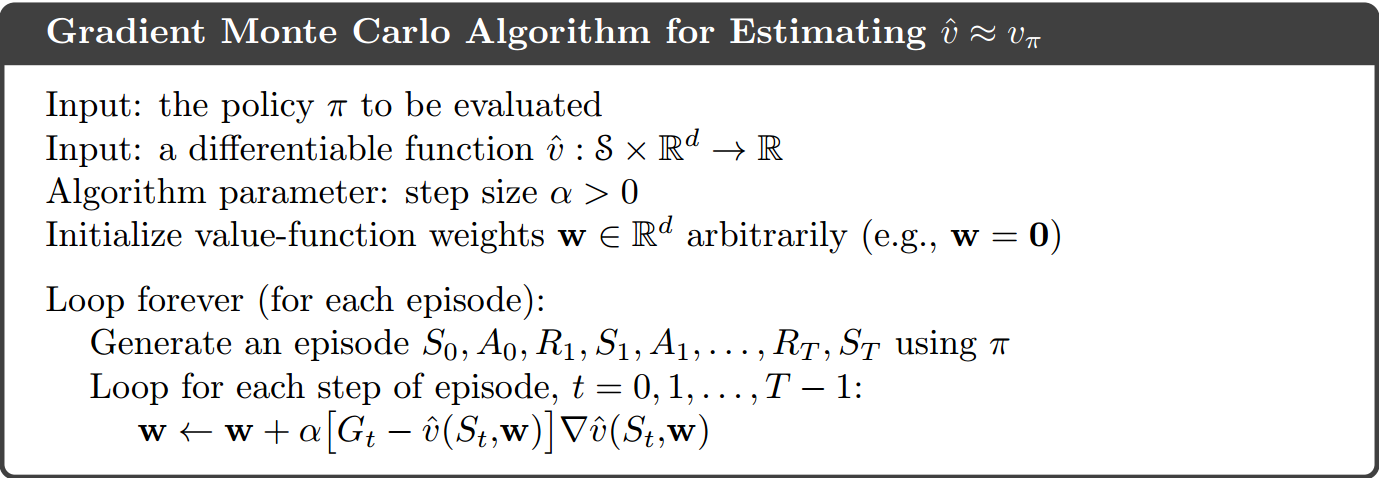
\includegraphics[scale = 0.3]{gradient_monte_carlo.png}}
\end{minipage}
\caption{\footnotesize{\textbf{Gradient Monte Carlo uses the SGD algorithm with Monte Carlo return estimate as target}}}
\label{fig: gradient_monte_carlo}
\end{figure}

\begin{figure}
\begin{minipage}[t]{1\linewidth}
  \centering
  \centerline{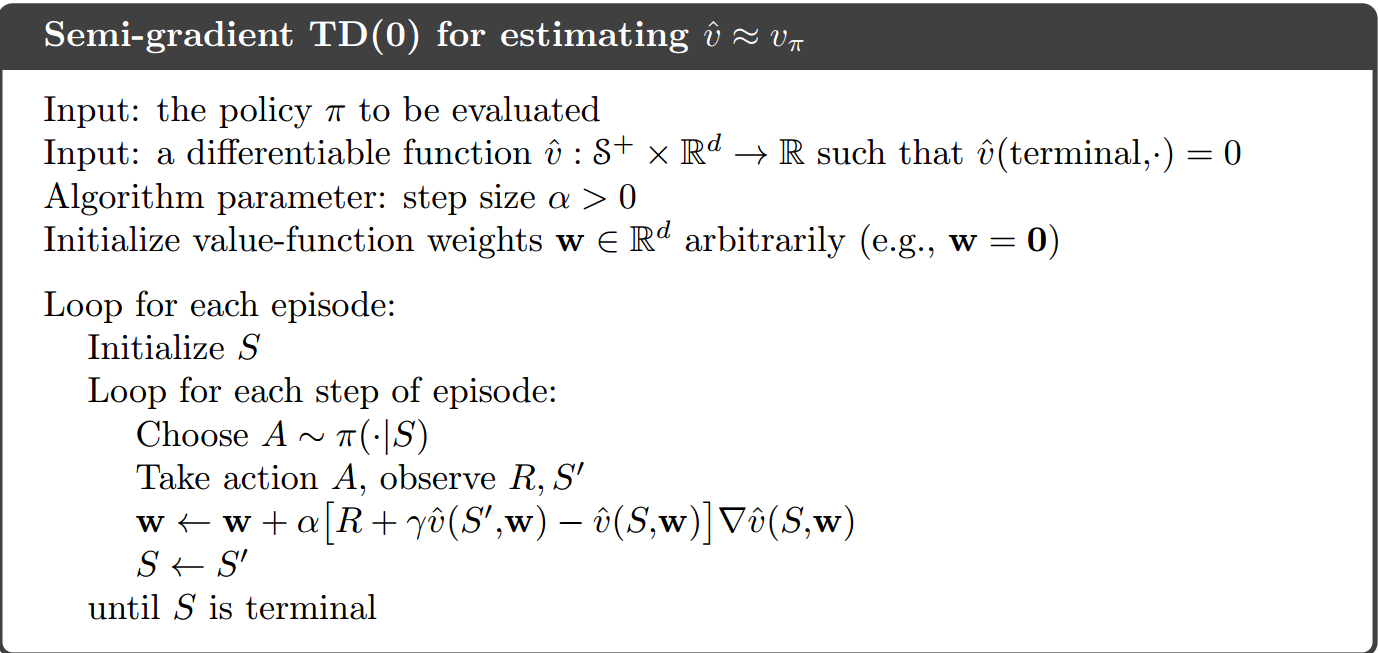
\includegraphics[scale = 0.3]{semi_grad_td_algo.png}}
\end{minipage}
\caption{\footnotesize{\textbf{Semi-gradient TD(0) algorithm}}}
\label{fig: semi_grad_td_algo}
\end{figure}

On the other hand, one \emph{does not obtain the same guarantees} if a \textbf{bootstrapping} estimate of $v_{\pi}(S_{t})$  is used as the target $\hat{G}_{t}$ as discussed in DP and TD algorithms. Bootstrapping methods are biased since they all depends on the estimation of value for successor states, which depends on the current value of the weight vector $\mb{w}_{t}$. Bootstrapping methods are \textbf{not} in fact instances of true gradient descent. They take into account the effect of changing the weight vector  $\mb{w}_{t}$ on the estimate, but \underline{ignore its effect on the target}. They include only a part of the gradient and, accordingly, we call them \emph{\textbf{semi-gradient methods}}. 

The \textbf{semi-gradient methods} with \textbf{TD(0) updates}:
\begin{align}
\mb{w}_{t+1} &\leftarrow  \mb{w}_{t} + \alpha \brac{R_{t+1} + \gamma \hat{v}(S_{t+1}, \mb{w}_{t}) - \hat{v}(S_{t}, \mb{w}_{t})} \grad{\mb{w}}{\hat{v}(S_{t}, \mb{w}_{t})} \label{eqn: td_fun_approx}
\end{align} Here $\delta_{t} = R_{t+1} + \gamma \hat{v}(S_{t+1}, \mb{w}_{t}) - \hat{v}(S_{t}, \mb{w}_{t})$ is the \textbf{TD error}. Figure \ref{fig: semi_grad_td_algo} describes the semi-gradient TD(0) methods for value approximation. Although semi-gradient (bootstrapping) methods do not converge as robustly as gradient methods, they do converge reliably in important cases such as the linear case discussed in the next section. Moreover, semi-gradient methods typically enable significantly faster learning since they can make update at each of each step instead of at the end of whole episode. 

Finally, we discuss a technique called \textbf{\emph{state aggregation}}. In state aggregation,  states are grouped together, with one estimated value (one component of the weight vector $\mb{w}$) for each group. The value of a state is estimated as its group’s component, and when the state is updated, that component alone is updated. This is a \textbf{binning method} to convert a large number of states into a lower dimensional weight vector $\mb{w}$ (dimension= no. of groups) in order to increase generalization. For SGD, note that $\brac{\grad{\mb{w}}{\hat{v}(S_{t}, \mb{w}_{t})}}_{j} = 1$ if the state $S_{t}$ belongs to the bin $j$, otherwise is zero. (i.e. group indicator function). Thus \eqref{eqn: td_fun_approx} becomes conventional TD(0) for states in the bin.

\section{Linear methods}
A simple form of value function approximation is \emph{\textbf{generalized linear approximation}}.
\begin{align}
\hat{v}(s, \mb{w}_{t}) &= \sum_{k}w_{k,t} \phi_{k}(s) = \inn{ \mb{w}_{t}}{\mb{\phi}(s)} \label{eqn: generalized_linear_form}
\end{align} where $\mb{w} = [w_{k,t}]$ is the function parameter, and $\set{\phi_{k}}$ is some \emph{\textbf{basis function}} defined on state-value functional space  $\cF:=\set{f: \cS \rightarrow \bR}$. $\mb{\phi}(s)$ is called a \textbf{\emph{feature vector}} representing state $s$. WIth \eqref{eqn: generalized_linear_form}, the SGD in \eqref{eqn: sgd_fun_approx} can be formulated as
\begin{align}
\mb{w}_{t+1} &\leftarrow  \mb{w}_{t} + \alpha \brac{\hat{G}_{t} - \hat{v}(S_{t}, \mb{w}_{t})} \mb{\phi}(S_{t}) \label{eqn: linear_sgd}
\end{align} since $\grad{}{\hat{v}(s, \mb{w}_{t})} = \mb{\phi}(s)$.  Note that the \textbf{tabular methods} can be formulated as linear methods with \textbf{indicator feature} (\textbf{one-hot encoding}) $\phi_{k}(s) = \ind{s = s_{k}}$. 

Due to its simple form, linear methods have strong convergence guarantee. In fact, there is only one optimum (or, in degenerate cases, one set of equally good optima), and thus any method that is guaranteed to converge to or near a \emph{local optimum} is automatically guaranteed to converge to or near the \textbf{global optimum}. In other words, the SGD method in \eqref{eqn: linear_sgd} converges to global optimal solution given that the value target is \emph{unbiased} and some stochastic conditions. The gradient Monte Carlo for linear approximation, for example, has the global optimality convergence results.  


The generalized linear approximation has \textbf{low variance} but \textbf{high bias} (bias-variance tradeoff). This means that for semi-gradient (boostrapping) methods, which use the linear estimates in the target function, do not converge to the global minimal. However, they do converge to a \textbf{fixed-point solution} 
\begin{align}
\mb{w}_{t+1} &\leftarrow  \mb{w}_{t} + \alpha \brac{R_{t+1} + \gamma  \inn{ \mb{w}_{t}}{\mb{\phi}(S_{t+1})}-  \inn{ \mb{w}_{t}}{\mb{\phi}(S_{t})}} \mb{\phi}(S_{t}) \label{eqn: linear_semi_grad_td} \\
&= \mb{w}_{t} + \alpha \brac{R_{t+1}\mb{\phi}_{t} - \mb{\phi}_{t}\paren{\mb{\phi}_{t} - \gamma \mb{\phi}_{t+1} }^{T}\mb{w}_{t} }\nonumber
\end{align} In expectation, it becomes
\begin{align*}
\E{}{\mb{w}_{t+1}|\mb{w}} &=\mb{w}_{t} + \alpha \paren{\mb{r} - \mb{A}\mb{w}_{t}} \\
&=\paren{\mb{I} - \alpha\mb{A}} \mb{w}_{t} + \alpha \mb{r} 
\end{align*} where $\mb{r} = \E{}{R_{t+1}\mb{\phi}_{t}}$ and $\mb{A} = \E{}{\mb{\phi}_{t}\paren{\mb{\phi}_{t} - \gamma \mb{\phi}_{t+1} }^{T}}$. When it converges, the fixed-point solution is
\begin{align*}
\mb{0}&= \mb{r} - \mb{A}\mb{w}_{t} \\
\mb{w}_{TD} &=  \mb{A}^{-1}\mb{r}
\end{align*} which is a linear projection of expected rewards.

\begin{theorem}
At the TD fixed point, the mean squared value error is within a bounded expansion of the lowest possible error:
\begin{align*}
\overline{VE}(\mb{w}_{TD}) &\le \frac{1}{1-\gamma} \overline{VE}(\mb{w}_{*})
\end{align*}
\end{theorem}
\begin{proof}
Note that $\mb{A} = \E{}{\mb{\phi}_{t}\paren{\mb{\phi}_{t} - \gamma \mb{\phi}_{t+1} }^{T}}$ where $ \mb{\phi}_{t+1} :=  \mb{\phi}(S_{t+1})$. Given the dynamic function and policy, we can be reformulated it as 
\begin{align*}
\mb{A} &= \sum_{s}\mu(s)\sum_{a}\pi(a|s) \sum_{s', r}p(s', r| s, a)\mb{\phi}(s)\paren{\mb{\phi}(s) - \gamma \mb{\phi}(s')}^{T}\\
&=  \sum_{s}\mu(s)\sum_{s'}p(s'|s)\mb{\phi}(s)\paren{\mb{\phi}(s) - \gamma \mb{\phi}(s')}^{T}\\
&= \sum_{s}\mu(s)\mb{\phi}(s)\brac{\mb{\phi}(s) - \gamma  \sum_{s'}p(s'|s)\mb{\phi}(s')}^{T} \\
&= \mb{\Phi}^{T}\mb{D}\brac{\mb{I} - \gamma \mb{P}}\mb{\Phi}
\end{align*} where $ \mb{\Phi} = [\mb{\phi}(s_{i})]_{1,\ldots,|\cS|}^{T} \in \bR^{|\cS| \times d}$ using $\mb{\phi}(s_{i})^{T}$ as its $i$-th row, $\mb{D} = \text{diag}\set{[\mu(s_{i})]_{1,\ldots,|\cS|}}  \in \bR^{|\cS| \times |\cS|}$ is the diagonal matrix of state distribution, $\mb{P} = [p(s'|s)]_{s,s' \in \cS} \in  \bR^{|\cS| \times |\cS|}$ is the state-transition matrix. 

The key is to show that $\mb{D}\brac{\mb{I} - \gamma \mb{P}} \succ \mb{0}$ is positive definite. Note that $\mb{D}$ is positive definite since its diagonal are all positive. The diagonal of  $\mb{D}\brac{\mb{I} - \gamma \mb{P}}$ is $\mu(s_{i})(1-p(s_{i}|s_{i})) = \mu(s_{i}) >0$. The off-diagonal is negative since $(-p(s_{i}|s_{j})) < 0$ and so all we have to show is that each row sum plus the corresponding column sum is positive. This is true since the state-transition matrix $\mb{P}$ is a stochastic matrix so the row sum is positive. (because $\mb{D}\brac{\mb{I} - \gamma \mb{P}}$ is symmetric real matrix and all of its diagonal entries are positive and greater than the sum of the absolute values of the corresponding off-diagonal entries) \QEDA
\end{proof}
Note that since the $\gamma$ is closer to $1$, the upper bound is very loose. 

This fixed-point solution applies to other on-policy bootstrapping methods as well. We can show that \textbf{linear semi-gradient dynamic programming} with updates according to the on-policy distribution also converge to the same fixed-point solution $\mb{w}_{TD}$.

\subsection{Choice of basis function / feature construction }
The choice of different basis function or features $\phi(s)$ will affect the ability of generalization and discrimination for the function approximation. We listed several important basis functions and feature mapping: 
\begin{itemize}
\item \textbf{Indicator function} (one-hot encoding): The simpliest feature mapping is one-hot encoding, which is essentially using each state value itself
\begin{align*}
\phi_{k}(\mb{s}) &:= \ind{\mb{s} = \mb{s}_{k}}, \quad \mb{s}_{k} \in \cS 
\end{align*} The main disadvantages for using one-hot encoding is that the \textbf{dimensionality} of the one-hot encoding increase exponentially when the state dimension increases. Suppose $\cS \subset \cR^{d}$ where $|\cR| = k$, then the one-hot encoding has dimension $k^d$. Also one-hot encoding can only be applied to \textbf{discrete state space}. For continous space, we have to use coarse coding or tile coding. 

The\textbf{ tabular methods} discussed before can be seen as \textbf{linear function approximation with one-hot encoding}. Due to sparisy of one-hot encoding, both SGD and semi-gradient methods can be easily computed by only updating weights corresponding to non-zero entries of one-hot encoding. This is essentially the same as MC, TD(0) etc. 
\begin{align*}
\text{SGD: }\mb{w}_{t+1,k} &\leftarrow  \mb{w}_{t, k} + \alpha \brac{\hat{G}_{t} - \hat{v}(S_{t}, \mb{w}_{t})}, \quad \text{only for k when }S_{t}=s_{k}\\
\text{TD(0): }\mb{w}_{t+1,k} &\leftarrow  \mb{w}_{t,k} + \alpha \brac{R_{t+1} + \gamma \mb{w}_{t,j} -  \mb{w}_{t,k}}, \quad \text{when }S_{t}=s_{k}, S_{t+1}=s_{j}
\end{align*}


\item \textbf{Polynomials, Fourier basis and RBF basis function}:  These are all different sets of classical functional basis for state function space $\cF$.  Using this basis as feature mapping, the function approximation for reinforcement learning is treated the same as the tasks of \textbf{interpolation} and \textbf{regression}. For $\mb{s} = (s_{1}, \ldots, s_{d})$, coefficient $\mb{c}_{k} = (c_{1,k}, \ldots, c_{d,k})$
\begin{align*}
\text{order-n Polynomial-basis: }\phi_{k}(\mb{s}) &:= \prod_{j=1}^{d}s_{j}^{c_{j,k}},\\
&s_{i} \in \bR \text{ and } c_{j,k} \in \set{0,\ldots, n},\;k=0,1,\ldots, (n+1)^d; \\
\text{Fourier: }\phi_{k}(\mb{s}) &:= \cos(\pi \mb{c}_{k}^{T}\mb{s}), \quad k=0,1,\ldots, \\
&s_{i} \in [0,1]\text{ and }c_{i,k} \in \set{0,\ldots, n}, k= 0, \ldots, (n+1)^d;\\
\text{Radical Basis Function (RBF): }\phi_{k}(\mb{s}) &:= \exp\paren{-\frac{\norm{\mb{s} - \mb{c}_{k}}{2}^{2}}{2\sigma_{k}^{2}}},\\
&s_{i} \in  \bR\text{ and }c_{i,k} \in  \bR, k= 0, \ldots, \infty
\end{align*}  In these cases, the feature vector $\mb{\phi}$ form a set of (linearly independent) basis for real-valued functional space $\cF=\set{f: \cS \rightarrow \bR}$ and the weight $\mb{w}$ becomes the \emph{coordinate} of the value function in the space $\cF$.



\item \textbf{Coarse Coding}: Coarse Coding is an extension of one-hot encoding to groups of states. Specifically, define a collection of subset regions $\set{U_{1}, \ldots, U_{M}}$ that \emph{\textbf{covers}} the state space so that $\cS \subset \bigcup_{i}U_{i}$ and $U_{i}\cap U_{j} \neq \emptyset$ for some $i\neq j$. The Coarse Coding features are defined as 
\begin{align*}
\phi_{k}(\mb{s}) &:= \ind{\mb{s} \in U_{k}}, \quad k=1,\ldots, M 
\end{align*} For feature vector $\mb{\phi}(\mb{s}) \in \{0,1\}^{M}$, the nonzero entries indicates the region index that covers the state $\mb{s}$.  
\begin{figure}
\begin{minipage}[t]{1\linewidth}
  \centering
  \centerline{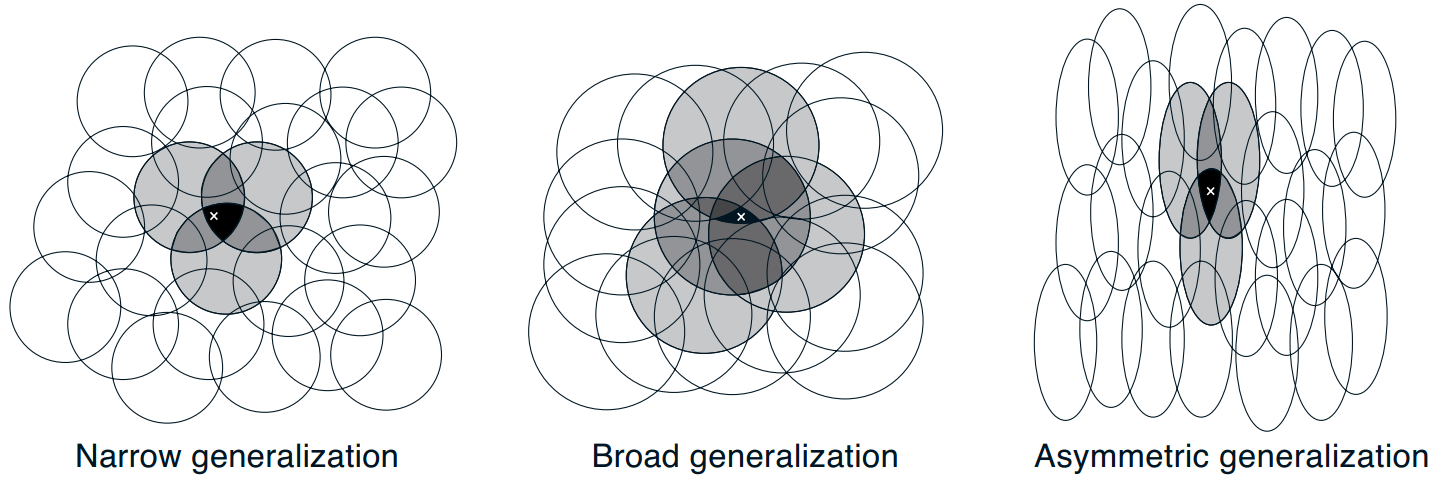
\includegraphics[scale = 0.3]{coarse_coding.png}}
\end{minipage}
\caption{\footnotesize{\textbf{coarse coding}}}
\label{fig: coarse_coding}
\end{figure}

The  \textbf{size} and the \textbf{shape} of collection of all region  that covers the state $\mb{s}$, i.e. $\bigcup_{\set{k: \mb{s} \in U_{k}}}U_{k}$, measures the \textbf{generalization} of the coarse encoding and  value approximation.  Note that all states within the same region $U_{k}$ shared the same feature $\phi_{k}$ and the same weight $\mb{w}_{k}$. So during the update, all of these states in the same region are updated simultaneously. These regions that cover $\mb{s}$ are seen as the receiptive fields of the state $\mb{s}$. In convolutional neural network, the region as well as the weight for each region are learned. CNN can be seen as a generalization of this idea. 

The \textbf{size} of non-empty overlapping of these regions $U_{i}\cap U_{j} \neq \emptyset$ measures the \textbf{discrimination} of the coarse coding and value approximation. Note that weights corresponding to $U_{i}$ and $U_{j}$ are updated independently. Thus, the smaller the overlapping region, the more \textbf{independent} the states in these two regions are. 

The \textbf{state aggregation} discussed above can be seen as a special case of coarse coding when $U_{i}\cap U_{j} = \emptyset$ for all $i,j$, i.e. $\set{U_1, \ldots, U_{M}}$ forms a \textbf{partition} of the state space. 

\item \textbf{Tile Coding}: Tile Coding is another way to \textbf{\emph{generalize}} the \emph{one-hot encoding} and \emph{state aggregation} methods. Consider a set of $H$ \textbf{tilings}. Each \underline{\emph{tiling}} defines a \textbf{partition} $\set{U^{h}_{1},\ldots, U^{h}_{M}}$ of the state space $\cS \subset \bigcup_{i}U^{h}_{i}$ and $U_{i}^{h}\cap U^{h}_{j} = \emptyset$ for all $i\neq j$. The element of tiling $U_{i}^{h}$ is called a \textbf{\emph{tile}}. The Tile Coding features are defined as 
\begin{align*}
\phi_{k, h}(\mb{s}) &:= \ind{\mb{s} \in U^{h}_{k}}, \quad k=1,\ldots, M,\quad h=1,\ldots, H.  
\end{align*} The feature vector  $\mb{\phi}(\mb{s}) := [\mb{\phi}_{1}(\mb{s}), \ldots, \mb{\phi}_{h}(\mb{s})] \in \{0,1\}^{M\, H}$ has dimension $M \times H$, where $\mb{\phi}_{l} := [\phi_{k, l}(\mb{s})]_{k=1,\ldots, M}$. Note that if $H=1$, we have \textbf{state aggretation} method. 
\begin{figure}
\begin{minipage}[t]{1\linewidth}
  \centering
  \centerline{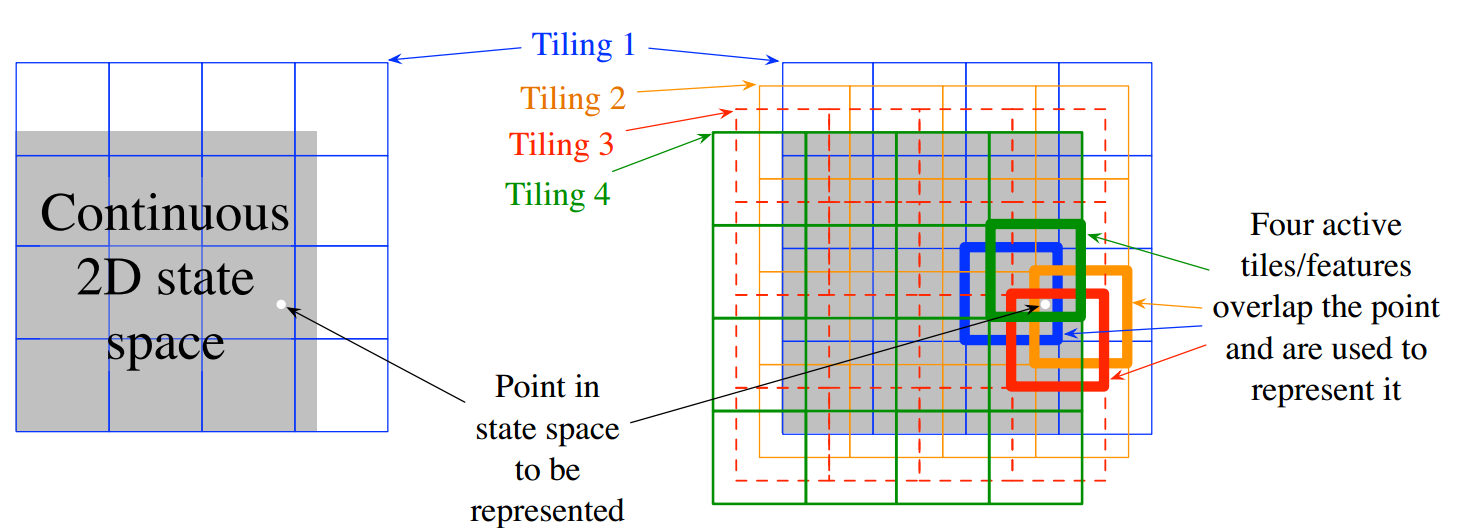
\includegraphics[scale = 0.3]{tile_coding.png}}
\end{minipage}
\caption{\footnotesize{\textbf{tile coding}}}
\label{fig: tile_coding}
\end{figure}

From Figure \ref{fig: tile_coding}, the tiles or receptive field here are \textbf{squares} rather than the circles in Figure \ref{fig: coarse_coding}. With just one tiling, the tile coding has less generalization compared to coarse coding, since two receptive fields within one tiling do not overlap. To increase overlapping, multiple tilings are used, each \textbf{offset} by a fraction of \textbf{a tile width}. Figure \ref{fig: tile_coding} shows the multiple tiling. 

An immediate practical advantage of tile coding is that, because it works with \emph{\textbf{partitions}}, the overall number of features that are \textbf{active} at one time is \textbf{the same for any state}. (i.e. for given $\mb{s}$, there exists only one $U^{h}_{i_{h}}$ that contains it, so $\mb{\phi}(\mb{s})$ has \textbf{exactly} $H$ non-zeros.) Exactly one feature is present in each tiling, so \textbf{the total number of features present is always the same as the number of tilings}. This allows the step-size parameter, $\alpha$, to be set in an easy, intuitive way.  For example, choosing $\alpha = \frac{1}{H}$, where $H$ is the number of tilings, results in exact one-trial learning. If the example $s \rightarrow v$ is trained on, then whatever the prior estimate, $\hat{v}(\mb{s}, \mb{w}_{t})$, the new estimate will be $\hat{v}(\mb{s}, \mb{w}_{t+1}) = v$. 

Similar to one-hot encoding, tile coding also gains \textbf{computational advantages} from its use of \textbf{binary} feature vectors. Because each component is either 0 or 1, the weighted sum making up the approximate value function \eqref{eqn: linear_sgd} or \eqref{eqn: linear_semi_grad_td} is almost trivial to compute. Rather than performing $d$ multiplications and additions, one simply computes the \textbf{indices} of the $n \ll d$ \textbf{active features} and then \textbf{adds up} the $n$ corresponding components of the weight vector.
\begin{align*}
\hat{v}(\mb{s}, \mb{w}_{t}) &= \sum_{k}w_{k,t} \phi_{k}(\mb{s}) = \sum_{\{i: \mb{s}\, \in\, U^{h}_{i}\}} w_{i, t}
\end{align*}

\textbf{Generalization} occurs to states other than the one trained if those states fall within any of \textbf{the same tiles}, proportional to the \emph{number of tiles in common}. Even the choice of \textbf{how to offset the tilings} from each other affects generalization. If $w$ denotes the tile width and $H$ the number of tilings, then $\frac{w}{H}$ is a \emph{\textbf{fundamental unit}}. Within small squares  $\frac{w}{H}$ on a side, all states activate the same tiles, have the same feature representation, and the same approximated value. If a state is moved by $\frac{w}{H}$ in any cartesian direction, the feature representation changes by one \emph{component}/tile.

We can also use non-square tiles. In choosing a tiling strategy, one has to pick the number of the tilings and the shape of the tiles. The number of tilings, along with the size of the tiles, determines the resolution or fineness of the asymptotic approximation, i.e. the \textbf{discrimination} power.

CNN is like a combination of coarse coding and tile coding since it has overlapping receiptive fields (coarse coding) and has stacked multiple filters (tile coding). 

\end{itemize}

\section{Function approximation via Artificial Neural Networks}
Artificial Neural Networks (ANNs) are widely used to as (universal) nonlinear function approximator. In this case, a neural network can be applied to construct the feature representation 
\begin{align*}
\phi_{k}(\mb{s}) &:= \mb{W}_{k}^{i+1}\sigma\paren{\mb{W}^{i}\mb{s} + \mb{b}^{i}} + \mb{b}_{k}^{i+1}, i=1,\ldots, h
\end{align*} 

Due to its complexity in structure, we only \textbf{highlights} the critical points when using neural networks as value function approximation $\hat{v}(s, \mb{w})$.
\begin{itemize}
\item Since a neural network consists of multiple layers, the weight $\mb{w} := (\mb{W}^{i}, \mb{b}^{i}, i=1,\ldots, h)$ consists of all weight matrix and bias term at each layer. 

\item The stochastic gradient descent and sem-gradient descent above still holds:
\begin{align*}
\mb{w}_{t+1} &\leftarrow  \mb{w}_{t} + \alpha \;\;\delta_{t} \grad{\mb{w}}{\hat{v}(S_{t}, \mb{w}_{t})}\\
\text{(SGD): }\delta_{t}&=\hat{G}_{t} - \hat{v}(S_{t}, \mb{w}_{t}) \\
\text{(Semi-gradient TD(0)): }\delta_{t}&= R_{t+1} + \gamma \hat{v}(S_{t+1}, \mb{w}_{t}) - \hat{v}(S_{t}, \mb{w}_{t})
\end{align*}

\item Due to its complexity and layer-wise graph structure, the computation in \textbf{each step} of SGD/Semi-gradient has two \textbf{procedures} (mulitple-step loops):
\begin{itemize}
\item \underline{\textbf{Forward pass}} (propagation): given $\mb{w}_{t}$ and $\mb{s}=S_{t}$, to \textbf{compute} $\hat{v}(S_{t}, \mb{w}_{t})$. This is the \textbf{inference} step. The error is computed via $\delta_{t}=\hat{G}_{t} - \hat{v}(S_{t}, \mb{w}_{t})$ if the sample return $\hat{G}_{t}$ is known. For TD(0), we have to compute two forward passes \textbf{simultaneously} in order to obtain \textbf{TD error}, i.e. $ \hat{v}(S_{t+1}, \mb{w}_{t})$, $ \hat{v}(S_{t}, \mb{w}_{t})$, for the state $S_{t}$ and its successor state $S_{t+1}$.

The time complexity of forward pass is determined by the total number of layers in neural network as well as all hidden layer dimensions.  

\item \underline{\textbf{Back-propagation}}: In back-propagation, the algorithm need to compute the \textbf{gradient} term $\grad{\mb{w}}{\hat{v}(S_{t}, \mb{w}_{t})}$ with respect to each weight matrices and bias terms in each layer. 

By using the \textbf{computation graph} and the \textbf{chain rule} of gradients, the algorithm can efficiently compute the gradient of each weight coefficient by one forward pass and one backward pass. Same as forward pass, the time complexity of forward pass is determined by the total number of layers in neural network as well as all hidden layer dimensions.  
\end{itemize}


\item For off-policy control with neural network, there is a significant issue with bootstrap \textbf{bias} and the \emph{\textbf{positive feedback loop}} that can cause. Q-learning estimates can diverge because of this. Note that the weight update in SGD as \eqref{eqn: sgd_fun_approx} is \textbf{not the same} as the SGD used for training neural network in supervised learning. In the latter case, the target function is \underline{fixed}, \underline{unknown} and the inputs are \underline{independent}, whereas the state $S_{t}$ and $S_{t+1}$ are  \underline{correlated} and the target $\hat{G}_{t}$ is  \underline{dynamic}, determined by samples or previous estimates. Thus the  \underline{convergence} of SGD/Semi-gradient algorithm for neural network function approximation is  \underline{not guaranteed}. 

The \textbf{Off-policy Divergence} is the main challenge for off-policy learning with function approximation—that the distribution of updates does not match the onpolicy distribution.

\item For TD error, we need to keep a copy old network $f(\mb{w}_{t-1})$ as well as the newly updated network $f(\mb{w}_t)$, since we need to use the old network for next state as well as old network for current state to construct the TD error.

\item For Q learning, \textbf{maximisation bias} is a problem, whereby the action chosen is more likely to have an over-estimate of its true value. This can be fixed by \textbf{double Q-learning}.

\item For Q-learning, using deep learning architecture we can learn complex value function. For instance the \textbf{\emph{Deep Q-Network (DQN)}} \citep{franccois2018introduction}  algorithm introduced by Mnih et al. (2015) is able to obtain strong performance in an online setting for a variety of ATARI games, directly by learning from the pixels. Check other deep RL models in \citep{franccois2018introduction}
\end{itemize}

\begin{figure}
\begin{minipage}[t]{1\linewidth}
  \centering
  \centerline{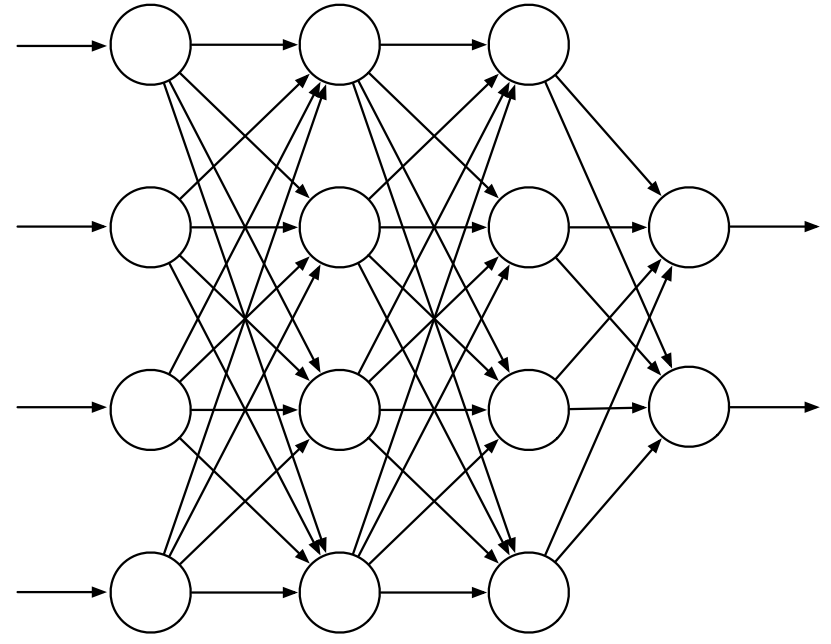
\includegraphics[scale = 0.3]{ANN.png}}
\end{minipage}
\caption{\footnotesize{\textbf{The artificial neural network}}}
\label{fig: tile_coding}
\end{figure}


\newpage
\bibliographystyle{plainnat}
\bibliography{reference.bib}
\end{document}